% Template LaTeX file for DAFx-10 papers
%
% To generate the correct references using BibTeX, run
%     latex, bibtex, latex, latex
% modified...
% - from DAFx-00 to DAFx-02 by Florian Keiler, 2002-07-08
% - from DAFx-02 to DAFx-03 by Gianpaolo Evangelista
% - from DAFx-05 to DAFx-06 by Vincent Verfaille, 2006-02-05
% - from DAFx-06 to DAFx-07 by Vincent Verfaille, 2007-01-05
%                          and Sylvain Marchand, 2007-01-31
% - from DAFx-07 to DAFx-08 by Henri Penttinen, 2007-12-12
%                          and Jyri Pakarinen 2008-01-28
% - from DAFx-08 to DAFx-09 by Giorgio Prandi, Fabio Antonacci 2008-10-03
% - from DAFx-09 to DAFx-10 by Hannes Pomberger 2010-02-01
% - from DAFx-10 to DAFx-12 by Jez Wells 2011
%
% Template with hyper-references (links) active after conversion to pdf
% (with the distiller) or if compiled with pdflatex.
%
% 20060205: added package 'hypcap' to correct hyperlinks to figures and tables
%                      use of \papertitle and \paperauthorA, etc for same title in PDF and Metadata
%
% 1) Please compile using latex or pdflatex.
% 2) If using pdflatex, you need your figures in a file format other than eps! e.g. png or jpg is working
% 3) Please use "paperftitle" and "pdfauthor" definitions below

%------------------------------------------------------------------------------------------
%  !  !  !  !  !  !  !  !  !  !  !  ! user defined variables  !  !  !  !  !  !  !  !  !  !  !  !  !  !
% Please use these commands to define title and author of the paper:
\def\papertitle{Templates for DAFx-13, Maynooth, Ireland}
\def\paperauthorA{The DAFx Crew and All Their Friends}
\def\paperauthorB{The Previous DAFx Crew}
\def\paperauthorC{Joseph Fourier}
\def\paperauthorD{Claude Shannon}


%------------------------------------------------------------------------------------------
\documentclass[twoside,a4paper]{article}
\usepackage{dafx_13}
\usepackage{amsmath,amssymb,amsfonts,amsthm}
\usepackage{euscript}
\usepackage[latin1]{inputenc}
\usepackage[T1]{fontenc}
\usepackage{ifpdf}

\usepackage[english]{babel}
\usepackage{caption}
\usepackage{subfig, color}

\setcounter{page}{1}
\ninept

\usepackage{times}
% Saves a lot of ouptut space in PDF... after conversion with the distiller
% Delete if you cannot get PS fonts working on your system.

% pdf-tex settings: detect automatically if run by latex or pdflatex
\newif\ifpdf
\ifx\pdfoutput\relax
\else
   \ifcase\pdfoutput
      \pdffalse
   \else
      \pdftrue
\fi

\ifpdf % compiling with pdflatex
  \usepackage[pdftex,
    pdftitle={\papertitle},
    pdfauthor={\paperauthorA, \paperauthorB, \paperauthorC, \paperauthorD},
    colorlinks=false, % links are activated as colror boxes instead of color text
    bookmarksnumbered, % use section numbers with bookmarks
    pdfstartview=XYZ % start with zoom=100% instead of full screen; especially useful if working with a big screen :-)
  ]{hyperref}
  \pdfcompresslevel=9
  \usepackage[pdftex]{graphicx}
  \usepackage[figure,table]{hypcap}
\else % compiling with latex
  \usepackage[dvips]{epsfig,graphicx}
  \usepackage[dvips,
    colorlinks=false, % no color links
    bookmarksnumbered, % use section numbers with bookmarks
    pdfstartview=XYZ % start with zoom=100% instead of full screen
  ]{hyperref}
  % hyperrefs are active in the pdf file after conversion
  \usepackage[figure,table]{hypcap}
\fi

\title{\papertitle}

%-------------SINGLE-AUTHOR HEADER STARTS (uncomment below if your paper has a single author)-----------------------
%\affiliation{
%\paperauthorA, \sthanks{This work was supported by the XYZ Foundation}}
%{\href{http://music.nuim.ie/}{Dept. of Music} \\ National University of Ireland\\ Maynooth, Irelabd\\
%{\tt \href{mailto:papers@dafx13.nuim.ie}{papers@dafx13.nuim.ie}
%}
%-----------------------------------SINGLE-AUTHOR HEADER ENDS------------------------------------------------------

%---------------TWO-AUTHOR HEADER STARTS (uncomment below if your paper has two authors)-----------------------
%\twoaffiliations{
%\paperauthorA, \sthanks{This work was supported by the XYZ Foundation}}
%{\href{http://music.nuim.ie/}{Dept. of Music} \\ National University of Ireland\\ Maynooth, Irelabd\\
%{\tt \href{mailto:papers@dafx13.nuim.ie}{papers@dafx13.nuim.ie}
%}
%{\paperauthorB, \sthanks{This guy is a very good fellow}}
%{\href{http://www.elec.york.ac.uk/research/audio.html}{Audio Lab, Department of Electronics} \\ University of York\\ York, UK\\
%{\tt \href{mailto:papers@dafx12.york.ac.uk}{papers@dafx12.york.ac.uk}}
%}
%-------------------------------------TWO-AUTHOR HEADER ENDS------------------------------------------------------

%---------------THREE-AUTHOR HEADER STARTS (uncomment below if your paper has three authors)-----------------------
%\threeaffiliations{
%\paperauthorA, \sthanks{This work was supported by the XYZ Foundation}}
%{\href{http://music.nuim.ie/}{Dept. of Music} \\ National University of Ireland\\ Maynooth, Irelabd\\
%{\tt \href{mailto:papers@dafx13.nuim.ie}{papers@dafx13.nuim.ie}
%}
%{\paperauthorB, \sthanks{This guy is a very good fellow}}
%{\href{http://www.elec.york.ac.uk/research/audio.html}{Audio Lab, Department of Electronics} \\ University of York\\ York, UK\\
%{\tt \href{mailto:papers@dafx12.york.ac.uk}{papers@dafx12.york.ac.uk}}
%}
%{\paperauthorC,\sthanks{Illustrious contributor}}
%{\href{http://dafx13.nuim.ie}{Spectral Labs } \\ Somewhere above the sky\\ {\tt \href{mailto:spectrum@sinus.oids}{mailto:spectrum@sinus.oids}}
%}

%-------------------------------------THREE-AUTHOR HEADER ENDS------------------------------------------------------

%----------------FOUR-AUTHOR HEADER STARTS (uncomment below if your paper has four authors)-----------------------
%\fouraffiliations{
%\paperauthorA, \sthanks{This work was supported by the XYZ Foundation}}
%{\href{http://music.nuim.ie/}{Dept. of Music} \\ National University of Ireland\\ Maynooth, Irelabd\\
%{\tt \href{mailto:papers@dafx13.nuim.ie}{papers@dafx13.nuim.ie}
%}
%{\paperauthorB, \sthanks{This guy is a very good fellow}}
%{\href{http://www.elec.york.ac.uk/research/audio.html}{Audio Lab, Department of Electronics} \\ University of York\\ York, UK\\
%{\tt \href{mailto:papers@dafx12.york.ac.uk}{papers@dafx12.york.ac.uk}}
%}
%{\paperauthorC,\sthanks{Illustrious contributor}}
%{\href{http://dafx13.nuim.ie}{Spectral Labs } \\ Somewhere above the sky\\ {\tt \href{mailto:spectrum@sinus.oids}{mailto:spectrum@sinus.oids}}
%}
%{\paperauthorD,\sthanks{Yes, senior}}
%{\href{http://dafx13.nuim.ie}{ Communications Office, Somewhere else} \\ Centre for Something \\ {\tt \href{mailto:some@where.no }{some@where.no}}
%}
%-------------------------------------FOUR-AUTHOR HEADER ENDS------------------------------------------------------

\begin{document}
% more pdf-tex settings:
\ifpdf % used graphic file format for pdflatex
  \DeclareGraphicsExtensions{.png,.jpg,.pdf}
\else  % used graphic file format for latex
  \DeclareGraphicsExtensions{.eps}
\fi

\maketitle

\begin{abstract}
This is the template file for the proceedings of the 16$^{\text{th}}$ International Conference on Digital Audio Effects (DAFx-13).
This template has been generated from WASPAA'99 templates and aims at producing conference proceedings in electronic form.
The format is essentially the one used for ICASSP conferences.
Please use either this \LaTeX{} or the accompanying Word formats when preparing your submission.
The templates are available in electronic form on the following website:
\\ \href{http://dafx13.nuim}{http://dafx13.nuim.ie}. Thanks!

\end{abstract}

\section{Introduction}
\label{sec:intro}
This template can be found on the conference website.

\subsection{Figures}
\label{ssec:figures}
All figures should be centred on the column (or page, if the figure spans both columns).
Figure captions (in italic) should follow each figure and have the format given in Figure \ref{fft_plot}.
\begin{figure}[ht]
\centerline{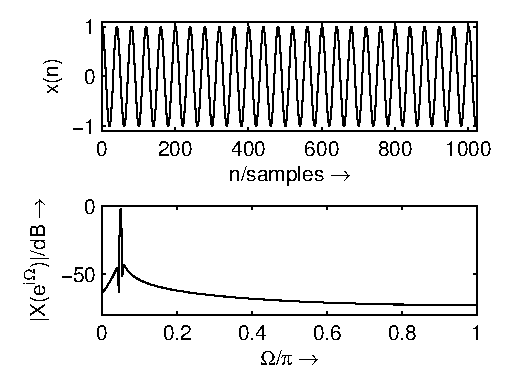
\includegraphics[scale=0.8]{fft_plot2.eps}}
\caption{\label{fft_plot}{\it Sinusoid in time and frequency domain.}}
\end{figure}
Vectorial figures are preferred. For example when using
\texttt{Matlab}, export using either Postscript or PDF format. Also,
in order to provide a better readability, figure text font size
should be at list identical to footnote font size. To do so using
\texttt{Matlab}, use the \texttt{subplot} command before plotting.
If bitmap figures are used, please make sure that the resolution is
enough for print quality. Fig. \ref{ftt_plot2} illustrates an
example of a figure spanning two columns.
\begin{figure*}[ht]
\center
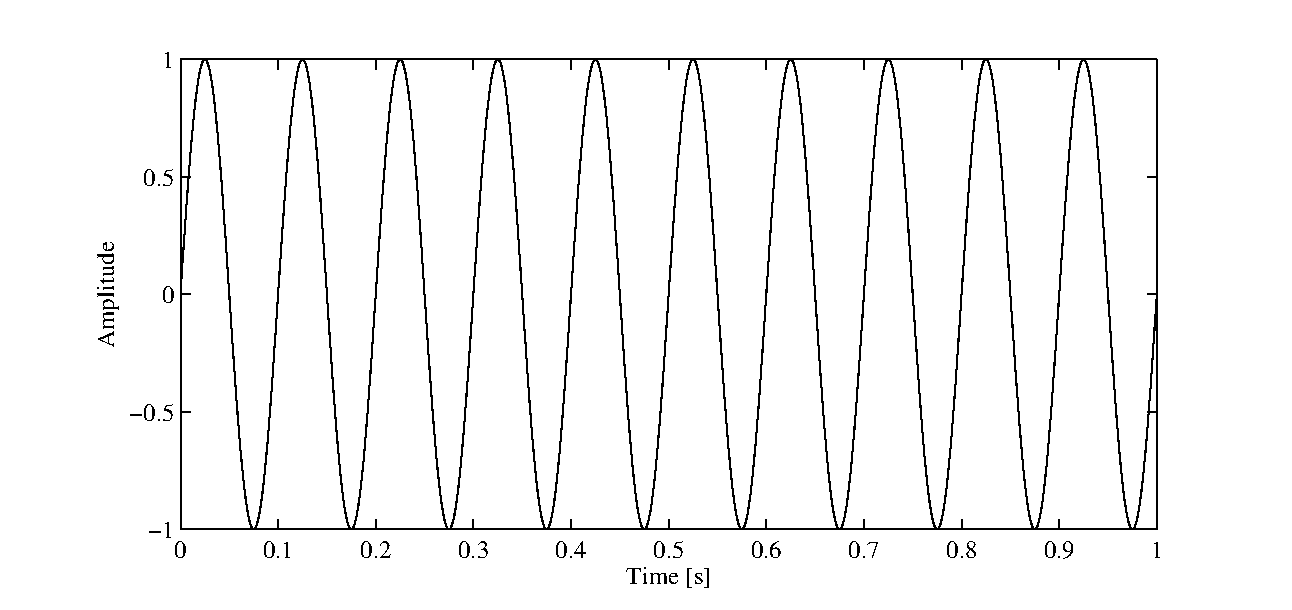
\includegraphics[width=5in]{TwoColumnSine2.eps} 
\caption{\label{ftt_plot2}{\it A figure spanning two columns, as mentioned in Sec. \ref{ssec:figures}. }}
\end{figure*} 

\subsection{Tables}
As for figures, all tables should be centred on the column (or page, if the table spans both columns).
Table captions should be in italic, precede each table and have the format given in Table \ref{tab:example}.

\begin{table}[htdp]
  \caption{{\it Basic trigonometric values.}}
  \begin{center}
    \begin{tabular}{|c|c|}\hline
        angle ($\theta$, rad) & $\sin \theta$ \\\hline
    $\frac{\pi}{2}$ & 1 \\
    $\pi$ & 0 \\
    $\frac{3\pi}{2}$ & -1 \\
    $2\pi$ & 0 \\\hline
    \end{tabular}
  \end{center}
  \label{tab:example}
\end{table}

\begin{table*}[htdp]
  \caption{{\it Basic trigonometric values, spanning two columns.}}
  \begin{center}
    \begin{tabular}{|c|c|c|c|c|c|c|}\hline
        angle ($\theta$, rad) & $\sin \theta$ & $\cos \theta $ & $(\sin \theta)/2 $ & $(\cos \theta) /2 $ & $(\sin \theta)/3 $ & $(\cos \theta)/3$    \\\hline
    $\frac{\pi}{2}$ & 1 & 0 & 1/2 & 0 & 1/3 & 0 \\
    $\pi$ & 0 & -1 & 0 & -1/2 & 0 & -1/3\\
    $\frac{3\pi}{2}$ & -1 & 0 & -1/2 & 0 & -1/3 & 0 \\
    $2\pi$ & 0 & 1 & 0 & 1/2 & 0 & 1/3\\\hline
    \end{tabular}
  \end{center}
  \label{tab:example2}
\end{table*}

\subsection{Equations}
Equations should be placed on separate lines and numbered:

\begin{equation}
X(e^{j\Omega})=\sum_{n=0}^{N-1}x(n)e^{-j\Omega n}
\label{eq1}
\end{equation}
where the sequence $x(n)$ in equation (\ref{eq1}) is a windowed frame:
\begin{equation}
x(n)=s(n) w(n)
\label{eq2}
\end{equation}
with a window function $w(n)$.

\subsection{Page Numbers}
Page numbers will be added to the document electronically, so {\em please leave the numbering as is},
that is, the first page will start at page DAFX-1 and the last page, at most, will have to be DAFX-8.

\subsection{References}
The references will be numbered in order of appearance \cite{Mitra:Kaiser:1993:DSP:handbook}, \cite{Haykin:1991:adaptive:filter}, \cite{Moorer:2000:AES:audio:millenium} and \cite{Nackaerts:2001:ICMC}. Please avoid listing references that do not appear in the text (we did the opposite in this template).

\subsubsection{Reference Format}
The reference format is the standard IEEE one. We recommend to use BibTeX to create the reference list.

\section{Conclusions}
This template can be found on the conference website.
For changing the number of author affiliations (1-4), uncomment the corresponding regions in the \texttt{DAFx13\_tmpl.tex} file.
Please, submit full-length papers (max.~8 pages both oral and poster presentations).
Submission is fully electronic and automated through the Conference Web Submission System.
DO NOT send us papers directly by e-mail.

\section{Acknowledgments}
Many thanks to the great number of anonymous reviewers!

%\newpage
\nocite{*}
\bibliographystyle{IEEEbib}
\bibliography{DAFx13_tmpl} % requires file DAFx13_tmpl.bib

\section{Appendix: Margin Check}
This section shows the column margins for the text. \bigskip\newline

Lorem ipsum dolor sit amet, consectetur adipisici elit, sed eiusmod tempor incidunt ut labore et dolore magna aliqua. Ut enim ad minim veniam, quis nostrud exercitation ullamco laboris nisi ut aliquid ex ea commodi consequat. Quis aute iure reprehenderit in voluptate velit esse cillum dolore eu fugiat nulla pariatur. Excepteur sint obcaecat cupiditat non proident, sunt in culpa qui officia deserunt mollit anim id est laborum.


Duis autem vel eum iriure dolor in hendrerit in vulputate velit esse molestie consequat, vel illum dolore eu feugiat nulla facilisis at vero eros et accumsan et iusto odio dignissim qui blandit praesent luptatum zzril delenit augue duis dolore te feugait nulla facilisi. Lorem ipsum dolor sit amet, consectetuer adipiscing elit, sed diam nonummy nibh euismod tincidunt ut laoreet dolore magna aliquam erat volutpat.

Ut wisi enim ad minim veniam, quis nostrud exerci tation ullamcorper suscipit lobortis nisl ut aliquip ex ea commodo consequat. Duis autem vel eum iriure dolor in hendrerit in vulputate velit esse molestie consequat, vel illum dolore eu feugiat nulla facilisis at vero eros et accumsan et iusto odio dignissim qui blandit praesent luptatum zzril delenit augue duis dolore te feugait nulla facilisi.

Nam liber tempor cum soluta nobis eleifend option congue nihil imperdiet doming id quod mazim placerat facer possim assum. Lorem ipsum dolor sit amet, consectetuer adipiscing elit, sed diam nonummy nibh euismod tincidunt ut laoreet dolore magna aliquam erat volutpat. Ut wisi enim ad minim veniam, quis nostrud exerci tation ullamcorper suscipit lobortis nisl ut aliquip ex ea commodo consequat.

Duis autem vel eum iriure dolor in hendrerit in vulputate velit esse molestie consequat, vel illum dolore eu feugiat nulla facilisis.

At vero eos et accusam et justo duo dolores et ea rebum. Stet clita kasd gubergren, no sea takimata sanctus est Lorem ipsum dolor sit amet. Lorem ipsum dolor sit amet, consetetur sadipscing elitr, sed diam nonumy eirmod tempor invidunt ut labore et dolore magna aliquyam erat, sed diam voluptua. At vero eos et accusam et justo duo dolores et ea rebum. Stet clita kasd gubergren, no sea takimata sanctus est Lorem ipsum dolor sit amet. Lorem ipsum dolor sit amet, consetetur sadipscing elitr, At accusam aliquyam diam diam dolore dolores duo eirmod eos erat, et nonumy sed tempor et et invidunt justo labore Stet clita ea et gubergren, kasd magna no rebum. sanctus sea sed takimata ut vero voluptua. est Lorem ipsum dolor sit amet. Lorem ipsum dolor sit amet, consetetur sadipscing elitr, sed diam nonumy eirmod tempor invidunt ut labore et dolore magna aliquyam erat.

Consetetur sadipscing elitr, sed diam nonumy eirmod tempor invidunt ut labore et dolore magna aliquyam erat, sed diam voluptua. At vero eos et accusam et justo duo dolores et ea rebum. Stet clita kasd gubergren, no sea takimata sanctus est Lorem ipsum dolor sit amet. Lorem ipsum dolor sit amet, consetetur sadipscing elitr, sed diam nonumy eirmod tempor invidunt ut labore et dolore magna aliquyam erat, sed diam voluptua. At vero eos et accusam et justo duo dolores et ea rebum. Stet clita kasd gubergren, no sea takimata sanctus est Lorem ipsum dolor sit amet. Lorem ipsum dolor sit amet, consetetur sadipscing elitr, sed diam nonumy eirmod tempor invidunt ut labore et dolore magna aliquyam erat, sed diam voluptua. At vero eos et accusam et justo duo dolores et ea rebum. Stet clita kasd gubergren, no sea takimata sanctus est Lorem ipsum dolor sit amet.

Lorem ipsum dolor sit amet, consectetur adipisici elit, sed eiusmod tempor incidunt ut labore et dolore magna aliqua. Ut enim ad minim veniam, quis nostrud exercitation ullamco laboris nisi ut aliquid ex ea commodi consequat. Quis aute iure reprehenderit in voluptate velit esse cillum dolore eu fugiat nulla pariatur. Excepteur sint obcaecat cupiditat non proident, sunt in culpa qui officia deserunt mollit anim id est laborum.


Duis autem vel eum iriure dolor in hendrerit in vulputate velit esse molestie consequat, vel illum dolore eu feugiat nulla facilisis at vero eros et accumsan et iusto odio dignissim qui blandit praesent luptatum zzril delenit augue duis dolore te feugait nulla facilisi. Lorem ipsum dolor sit amet, consectetuer adipiscing elit, sed diam nonummy nibh euismod tincidunt ut laoreet dolore magna aliquam erat volutpat.

Ut wisi enim ad minim veniam, quis nostrud exerci tation ullamcorper suscipit lobortis nisl ut aliquip ex ea commodo consequat. Duis autem vel eum iriure dolor in hendrerit in vulputate velit esse molestie consequat, vel illum dolore eu feugiat nulla facilisis at vero eros et accumsan et iusto odio dignissim qui blandit praesent luptatum zzril delenit augue duis dolore te feugait nulla facilisi.

Nam liber tempor cum soluta nobis eleifend option congue nihil imperdiet doming id quod mazim placerat facer possim assum. Lorem ipsum dolor sit amet, consectetuer adipiscing elit, sed diam nonummy nibh euismod tincidunt ut laoreet dolore magna aliquam erat volutpat. Ut wisi enim ad minim veniam, quis nostrud exerci tation ullamcorper suscipit lobortis nisl ut aliquip ex ea commodo consequat.

Duis autem vel eum iriure dolor in hendrerit in vulputate velit esse molestie consequat, vel illum dolore eu feugiat nulla facilisis.

At vero eos et accusam et justo duo dolores et ea rebum. Stet clita kasd gubergren, no sea takimata sanctus est Lorem ipsum dolor sit amet. Lorem ipsum dolor sit amet, consetetur sadipscing elitr, sed diam nonumy eirmod tempor invidunt ut labore et dolore magna aliquyam erat, sed diam voluptua. At vero eos et accusam et justo duo dolores et ea rebum. Stet clita kasd gubergren, no sea takimata sanctus est Lorem ipsum dolor sit amet. Lorem ipsum dolor sit amet, consetetur sadipscing elitr, At accusam aliquyam diam diam dolore dolores duo eirmod eos erat, et nonumy sed tempor et et invidunt justo labore Stet clita ea et gubergren, kasd magna no rebum. sanctus sea sed takimata ut vero voluptua. est Lorem ipsum dolor sit amet. Lorem ipsum dolor sit amet, consetetur sadipscing elitr, sed diam nonumy eirmod tempor invidunt ut labore et dolore magna aliquyam erat.

Consetetur sadipscing elitr, sed diam nonumy eirmod tempor invidunt ut labore et dolore magna aliquyam erat, sed diam voluptua. At vero eos et accusam et justo duo dolores et ea rebum. Stet clita kasd gubergren, no sea takimata sanctus est Lorem ipsum dolor sit amet. Lorem ipsum dolor sit amet, consetetur sadipscing elitr, sed diam nonumy eirmod tempor invidunt ut labore et dolore magna aliquyam erat, sed diam voluptua. At vero eos et accusam et justo duo dolores et ea rebum. Stet clita kasd gubergren, no sea takimata sanctus est Lorem ipsum dolor sit amet. 
\end{document}
